\section{Quantitative convergence on the triangle and square}\label{sec:cyclequant}

The preceding sections prove the classification. We now measure the gap between finite-order feasibility and compatibility on the triangle and square. The parity witness of Section~\ref{sec:cycles} gives an initial lower bound; a modification of its unconstrained Fourier coefficients improves it to $\Omega(1/t)$. A convex-order argument supplies the upper bound, and the final two subsections compare the hierarchy orders and finite thresholds.

\subsection{A corrected density and a linear lower bound}\label{sec:corrected}

The density \eqref{eq:Hdensity} fixes every auxiliary character, including characters that no prescription refers to. Changing those characters restores positivity at a larger $q$.

\begin{lemma}[Phase telescoping]\label{lem:telescope}
For real $\theta_1,\dots,\theta_m$,
\[
1-\cos\Bigl(\sum_{g=1}^m\theta_g\Bigr)\ \le\ m\sum_{g=1}^m\bigl(1-\cos\theta_g\bigr).
\]
\end{lemma}

\begin{proof}
$1-\cos\phi=\tfrac12|1-e^{i\phi}|^2$, and
$1-\prod_ge^{i\theta_g}=\sum_g\bigl(\prod_{g'<g}e^{i\theta_{g'}}\bigr)(1-e^{i\theta_g})$,
so $|1-\prod_ge^{i\theta_g}|\le\sum_g|1-e^{i\theta_g}|$. Cauchy--Schwarz gives $\bigl(\sum_g a_g\bigr)^2\le m\sum_ga_g^2$.
\end{proof}

\begin{lemma}[Corrected density]\label{lem:corrected}
Fix $m\in\{3,4\}$, $t\ge1$ and $0<q\le1/(16t)$, and set $c=4$ for $m=3$ and $c=5$ for $m=4$. On $m$ families of $t$ signs $s_{g,i}$ put
\begin{equation}\label{eq:Wdensity}
f_g=\prod_{i=1}^t\bigl(1+\mathrm{i}\sqrt q\,s_{g,i}\bigr),\qquad R=(1+q)^{t/2},\qquad
W(s)=\Real\prod_{g=1}^mf_g+c\sum_{g=1}^m\bigl(1-\Real f_g\bigr).
\end{equation}
Then $W$ is a real polynomial in $q$ with rational coefficients, $W\ge3/5$ for $m=3$ and $W\ge1/3$ for $m=4$, the law $\rho=2^{-mt}W$ is a probability law, and its characters are
\begin{equation}\label{eq:Wmoments}
\E_\rho\Bigl[\prod_{w\in S}s_w\Bigr]=
\begin{cases}
0,&|S|\text{ odd},\\
(1-c)(-q)^{|S|/2},&S\ne\varnothing\text{ even, inside one family},\\
(-q)^{|S|/2},&|S|\text{ even, meeting at least two families}.
\end{cases}
\end{equation}
\end{lemma}

\begin{proof}
Here $\mathrm{i}^2=-1$. Taking real parts keeps only even powers of $\mathrm{i}\sqrt q$, so $W$ is a real polynomial in $q$. Since $|1+i\sqrt q\,s|=(1+q)^{1/2}$ we may write $f_g=Re^{i\theta_g}$, and then
\[
\begin{aligned}
W&=R^m\cos\Bigl(\sum_g\theta_g\Bigr)+c\sum_g\bigl(1-R\cos\theta_g\bigr)\\
&=R^m-cm(R-1)-R^m\Bigl(1-\cos\sum_g\theta_g\Bigr)+cR\sum_g\bigl(1-\cos\theta_g\bigr).
\end{aligned}
\]
Lemma~\ref{lem:telescope} gives
\[
W\ \ge\ R^m-cm(R-1)+\bigl(cR-mR^m\bigr)\sum_g\bigl(1-\cos\theta_g\bigr).
\]
From $tq\le1/16$ we get $R^2=(1+q)^t\le\sum_{j\ge0}(tq)^j\le16/15$ and $R-1=(R^2-1)/(R+1)\le1/30$. For $m=3$, $c=4$: $3R^3\le4R$ because $3R^2\le16/5\le4$, and $W\ge1-12/30=3/5$. For $m=4$, $c=5$: $4R^4\le5R$ because $4R^3\le4(16/15)^{3/2}<5$, and $W\ge1-20/30=1/3$.

For the characters, work under the uniform law on the sign cube, where the families are independent and $\E f_g=1$. For $S$ with parts $S_g$ in the families,
\[
\E\Bigl[\prod_gf_g\prod_{w\in S}s_w\Bigr]=\prod_g\E\Bigl[f_g\prod_{w\in S_g}s_w\Bigr]=(i\sqrt q)^{|S|},
\]
whose real part is $0$ for odd $|S|$ and $(-q)^{|S|/2}$ for even $|S|$. Also $\E[(1-\Real f_g)\prod_{w\in S}s_w]$ vanishes unless $S$ is a nonempty subset of family $g$, in which case it equals $-\Real(i\sqrt q)^{|S|}$. Adding the contributions gives \eqref{eq:Wmoments}; the case $S=\varnothing$ gives $\E_\rho1=1$.
\end{proof}

\begin{theorem}[The square at $q=\Theta(1/t)$]\label{thm:squarelinear}
For every $t\ge1$ and every $0<q\le1/(16t)$, the square parity law $P_q$ of \eqref{eq:squaretarget} lies in $\IAI_t(\square)=\Iexp_t(\square)$.
\end{theorem}

\begin{proof}
Take $m=4$ and $c=5$ in Lemma~\ref{lem:corrected}, name the four families $x,y,z,w$ after the sources $X,Y,Z,W$, and define every copied observation by
\[
A^{il}=x_iw_l,\qquad B^{ij}=x_iy_j,\qquad C^{jk}=y_jz_k,\qquad D^{kl}=z_kw_l,
\]
that is by \eqref{eq:cyclewitness} for $m=4$. The density \eqref{eq:Wdensity} is symmetric within each family, so the law is invariant under independent permutations of the copy indices of each source. By Lemma~\ref{lem:boundary} every boundary occurring in an AI prescription, and every boundary of a subset of one of its blocks, is empty or meets at least two families; by \eqref{eq:Wmoments} such characters take the value $(-q)^{|\partial\cdot|/2}$, unchanged from \eqref{eq:masterchar}. The computation of Lemma~\ref{lem:cyclewitness} therefore applies verbatim: every injectable set has the marginal of $P_{4,q}=P_q$, ancestrally independent injectable blocks are independent, and the diagonal law is $P_q^{\otimes t}$. The moments that Lemma~\ref{lem:corrected} changed are the nonempty even characters inside a single family, and no prescription refers to one. Lemma~\ref{lem:rootsink} gives the recursive prescriptions.
\end{proof}

\begin{theorem}[The triangle at $q=\Theta(1/t)$]\label{thm:trianglelinear}
For every $t\ge1$ and every $0<q\le1/(16t)$, the parity-even law $\Pi(-q,-q,-q)$ of \eqref{eq:paritylaw} lies in $\IAI_t(\triangle)=\Iexp_t(\triangle)$.
\end{theorem}

\begin{proof}
Take $m=3$ and $c=4$ in Lemma~\ref{lem:corrected}, name the three families $x,y,z$ after the sources $X,Y,Z$, and define
\[
A^{ij}=x_iz_j,\qquad B^{ik}=x_iy_k,\qquad C^{jk}=z_jy_k,
\]
which is \eqref{eq:cyclewitness} for $m=3$ in the index convention of Section~\ref{sec:setup}. Positivity and normalization are Lemma~\ref{lem:corrected} with $W\ge3/5$. Symmetry within each family is again immediate. By Lemma~\ref{lem:boundary} every character prescribed by an injectable marginal, by an ancestrally independent product, or by the diagonal law has boundary empty or meeting at least two families, so \eqref{eq:Wmoments} returns $(-q)^{|\partial\cdot|/2}$ and the argument of Lemma~\ref{lem:cyclewitness} applies unchanged. The original copied triangle has $\E A=\E[x_iz_j]=-q$ and likewise $\E B=\E C=-q$, while $ABC=x_iz_jx_iy_kz_jy_k=1$, so its law is $\Pi(-q,-q,-q)=P_{3,q}$. Lemma~\ref{lem:rootsink} gives the recursive prescriptions.
\end{proof}
The exact certificates described in Section~\ref{sec:repro} check the square and triangle witnesses of the two theorems, with and without the flips of Corollaries~\ref{cor:squaredistance} and~\ref{cor:triangledistance}, at orders one and two for the square and one to three for the triangle: positivity of every atom, symmetry, the full diagonal law and every ancestral-independence prescription.


\subsection{Distance and the worst-case profile}\label{sec:worstcase}

For $H\in\{\mathrm{NW},\mathrm{AI},\mathrm{exp}\}$ and a pair-source scenario $G$ set
\begin{equation}\label{eq:Hprofile}
H^H_t(G)=\sup_{P\in\mathcal I^H_t(G)}d_{\TV}(P,\Cscen{G}),
\end{equation}
the worst-case total-variation distance from compatibility of a law the order-$t$ test accepts, with $d_{\TV}$ half the $\ell^1$ distance as in Section~\ref{sec:setup}.

\begin{lemma}[Max-moment inequality for the square]\label{lem:maxmoment}
Every $P\in\Csq$ in sign notation satisfies
\[
\max\{\E A,\ \E B,\ \E[AB]\}+4\,P(ABCD=-1)\ \ge\ 0 .
\]
\end{lemma}

\begin{proof}
Absorb the response seeds into incident sources, so $A=A(X,W)$, $B=B(X,Y)$, $C=C(Y,Z)$, $D=D(Z,W)$ are deterministic signs and $X,Y,Z,W$ are independent. Fix $z$ and write $g_z(Y)=C(Y,z)$, $h_z(W)=D(z,W)$ and
\[
\delta_z=\Pr\bigl(A(X,W)B(X,Y)\ne g_z(Y)h_z(W)\bigr),
\]
so that $\E_Z\delta_Z=P(ABCD=-1)=:\delta$. Put
\[
u_z(x)=\E_W\bigl[A(x,W)h_z(W)\bigr],\qquad v_z(x)=\E_Y\bigl[B(x,Y)g_z(Y)\bigr].
\]
Since $Y$ and $W$ are independent, $\E[ABg_zh_z\mid X=x]=u_z(x)v_z(x)$, and as $ABg_zh_z$ is a sign, $\E_X[1-u_zv_z]=2\delta_z$.

Let $f_z(x)=\sgn(u_z(x)+v_z(x))$, with $\sgn0=1$, and compare $A$ and $B$ with $A'_z=f_z(X)h_z(W)$ and $B'_z=f_z(X)g_z(Y)$. Then
\[
e_z:=\Pr(A\ne A'_z)+\Pr(B\ne B'_z)=\E_X\Bigl[1-\tfrac12|u_z+v_z|\Bigr]\le\E_X\bigl[1-u_zv_z\bigr]=2\delta_z,
\]
using $|u+v|\ge2uv$ on $[-1,1]^2$. Independence of $X,Y,W$ gives
\[
(\E A'_z)(\E B'_z)(\E[A'_zB'_z])=(\E f_z)^2(\E g_z)^2(\E h_z)^2\ \ge\ 0,
\]
so at least one of the three comparison moments is nonnegative. Each differs from the corresponding moment of $P$ by at most $2e_z$, since $|\E U-\E V|\le2\Pr(U\ne V)$ for signs and $\Pr(AB\ne A'_zB'_z)\le\Pr(A\ne A'_z)+\Pr(B\ne B'_z)$. Hence
\[
\max\{\E A,\E B,\E[AB]\}\ \ge\ -2e_z\ \ge\ -4\delta_z .
\]
The left side does not depend on $z$; averaging over $z$ finishes the proof.
\end{proof}

\begin{corollary}[Full-support survivors on the square]\label{cor:squaredistance}
$d_{\TV}(P_q,\Csq)\ge q/6$ for $0<q\le3-2\sqrt2$. With flip probability $\eta=q/64$ applied to each of the four bits and to every copied observation, $\widetilde P_q=T_\eta^{\otimes4}P_q$ is strictly positive, lies in $\IAI_t(\square)=\Iexp_t(\square)$ for $q\le1/(16t)$, and satisfies $d_{\TV}(\widetilde P_q,\Csq)\ge5q/48$. At $q_t=1/(16t)$,
\[
H^{\mathrm{exp}}_t(\square)=H^{\mathrm{AI}}_t(\square)\ \ge\ \frac5{768\,t}.
\]
\end{corollary}

\begin{proof}
If $R\in\Csq$ and $d=d_{\TV}(P_q,R)$, each of $\E_RA$, $\E_RB$, $\E_R[AB]$ is at most $-q+2d$ and the parity error of $R$ is at most $d$, since $P_q$ has none. Lemma~\ref{lem:maxmoment} gives $0\le-q+2d+4d$, so $d\ge q/6$. The noise argument of Theorem~\ref{thm:cycle} applies to the witness of Theorem~\ref{thm:squarelinear}, and $d_{\TV}(\widetilde P_q,P_q)\le4\eta=q/16$, so $d_{\TV}(\widetilde P_q,\Csq)\ge q/6-q/16=5q/48$. Substituting $q_t=1/(16t)$ gives $5/(768t)$, and Lemma~\ref{lem:rootsink} identifies the two suprema.
\end{proof}

\begin{corollary}[Full-support survivors on the triangle]\label{cor:triangledistance}
$d_{\TV}(\Pi(-q,-q,-q),\Ctri)\ge q/10$ for $0<q\le1/3$. With flip probability $\eta=q/192$ on each of the three bits and on every copied observation, the noisy target is strictly positive, lies in $\IAI_t(\triangle)=\Iexp_t(\triangle)$ for $q\le1/(16t)$, and is at distance at least $27q/320$ from $\Ctri$. At $q_t=1/(16t)$,
\[
H^{\mathrm{exp}}_t(\triangle)=H^{\mathrm{AI}}_t(\triangle)\ \ge\ \frac{27}{5120\,t}.
\]
\end{corollary}

\begin{proof}
The distance bound is Lemma~\ref{lem:cycledistance} for $m=3$, whose proof uses only Lemma~\ref{lem:quantrigidity} on the triangle itself. The three flips cost at most $3\eta=q/64$ in total variation, and $q/10-q/64=27q/320$. Feasibility is Theorem~\ref{thm:trianglelinear} with the noise argument of Theorem~\ref{thm:cycle}. Substituting $q_t=1/(16t)$ gives $27/(5120t)$.
\end{proof}

\subsection{A convex-order upper bound}\label{sec:convexorder}

Figure~\ref{fig:convex-order} summarizes the two ways of sampling a table used in the proof.

\begin{theorem}[Convex order along the diagonal]\label{thm:convexorder}
Let $G$ be a correlation scenario, that is, finitely many independent latent sources and observed variables with finite alphabets, each a stochastic function of the sources it reads, with $K$ joint outcomes; the order-$n$ inflation and the set $\INW_n(G)$ are defined as in Section~\ref{sec:pairsource} with sources in place of edges. Let $P\in\INW_n(G)$ with witness $\Gamma$. For a deterministic table $\omega$ of copied observations let $q_\omega$ be the observed law obtained by sampling one copy index uniformly and independently for each source and reading $\omega$ at those indices. Then $q_\omega\in\Cscen{G}$ for every $\omega$, and for every convex $\Phi$ on the observed simplex
\begin{equation}\label{eq:convexorder}
\E_\Gamma\,\Phi(q_\omega)\ \le\ \E\,\Phi(\widehat P_n),
\end{equation}
where $\widehat P_n$ is the empirical law of $n$ independent draws from $P$. In particular
\begin{equation}\label{eq:convexl2}
\E_\Gamma\|q_\omega-P\|_2^2\ \le\ \frac{1-\|P\|_2^2}{n},
\qquad
H^{\mathrm{NW}}_n(G)\ \le\ \min\Bigl\{1,\ \frac{\sqrt{K-1}}{2\sqrt n}\Bigr\}.
\end{equation}
\end{theorem}

\begin{proof}
Fix $\omega$. Sampling an index $I_e\in[n]$ uniformly and independently for each source $e$ and letting each observed variable $v$ output $\omega_v\bigl((I_e)_{e\ni v}\bigr)$, where $e\ni v$ ranges over the sources $v$ reads, is a model of $G$ with independent sources $I_e$ and deterministic responses, so $q_\omega\in\Cscen{G}$.

Draw one uniform permutation $\pi_e$ of $[n]$ for each source, independently of each other and of $\omega\sim\Gamma$, and set
\[
T_\ell=\Bigl(\omega_v\bigl((\pi_e(\ell))_{e\ni v}\bigr)\Bigr)_{v},\qquad \ell\in[n],
\qquad \widehat P=\frac1n\sum_{\ell=1}^n\delta_{T_\ell}.
\]
For each fixed choice of permutations, the symmetry of $\Gamma$ carries $(T_1,\dots,T_n)$ to the diagonal rows, so $(T_1,\dots,T_n)\sim P^{\otimes n}$; this remains true after averaging over the permutations, so $\widehat P$ has the law of $\widehat P_n$. Conditionally on $\omega$ and on a fixed $\ell$, the indices $(\pi_e(\ell))_e$ are independent and uniform on $[n]$, so $\E[\delta_{T_\ell}\mid\omega]=q_\omega$ and hence $\E[\widehat P\mid\omega]=q_\omega$. Conditional Jensen gives $\Phi(q_\omega)\le\E[\Phi(\widehat P)\mid\omega]$, and averaging over $\omega$ gives \eqref{eq:convexorder}.

Take $\Phi(\mu)=\|\mu-P\|_2^2$. Then $\E\|\widehat P_n-P\|_2^2=\frac1n\sum_xP(x)(1-P(x))=(1-\|P\|_2^2)/n$, which is the first part of \eqref{eq:convexl2}. Some $\omega$ attains at most the mean, and its $q_\omega$ is compatible, so
\[
d_{\TV}(P,\Cscen{G})\le\tfrac12\|P-q_\omega\|_1\le\frac{\sqrt K}2\|P-q_\omega\|_2\le\frac{\sqrt K}2\sqrt{\frac{1-\|P\|_2^2}n}\le\frac{\sqrt{K-1}}{2\sqrt n},
\]
using $\|P\|_2^2\ge1/K$. Total variation never exceeds $1$.
\end{proof}

\begin{figure}[htbp]
\centering
\begin{tikzpicture}[box/.style={draw,rounded corners=1mm,align=center,font=\small,inner sep=7pt}]
\node[box] (table) at (0,0) {Draw a table\\$\omega\sim\Gamma$};
\node[box] (emp) at (7,1.05) {Permute each source's indices\\read $n$ rows: $\widehat P$\\$\widehat P\overset{d}{=}\widehat P_n$};
\node[box] (comp) at (7,-1.05) {Sample source indices independently\\compatible law $q_\omega\in\mathcal C_G$};
\draw[-{Latex}] (table.east)--(emp.west);
\draw[-{Latex}] (table.east)--(comp.west);
\draw[-{Latex},inkblue] (emp.south)--node[right,font=\small] {$\mathbb E[\widehat P\mid\omega]=q_\omega$}(comp.north);
\end{tikzpicture}
\caption{The conditional expectation behind the convex-order bound. The same table yields an empirical distribution through permuted diagonal rows and a compatible law through independent source indices. Conditional Jensen compares their convex functionals. Squared Euclidean distance then gives the source-count-independent bound.}\label{fig:convex-order}
\end{figure}


The sampling mechanism is that of the finite de Finetti estimate of \cite[Section 4.2 and eq.~(A7)]{NW2020}, which bounds the same quantity by $L(1-\|P\|_2^2)/n$ for $L$ sources through the collision probability of two index samples. Using the full diagonal law through a conditional expectation, rather than its first two degrees, removes the factor $L$. Section~\ref{sec:general} draws the rejecting-order consequence.

\begin{corollary}[Brackets for the square and the triangle]\label{cor:brackets}
For every $t\ge1$,
\[
\frac5{768\,t}\ \le\ H^{\mathrm{exp}}_t(\square)=H^{\mathrm{AI}}_t(\square)\ \le\ H^{\mathrm{NW}}_t(\square)\ \le\ \min\Bigl\{1,\frac{\sqrt{15}}{2\sqrt t}\Bigr\},
\]
\[
\frac{27}{5120\,t}\ \le\ H^{\mathrm{exp}}_t(\triangle)=H^{\mathrm{AI}}_t(\triangle)\ \le\ H^{\mathrm{NW}}_t(\triangle)\ \le\ \frac{\sqrt7}{2\sqrt t}.
\]
\end{corollary}

\begin{proof}
Combine Corollaries~\ref{cor:squaredistance} and~\ref{cor:triangledistance} with Theorem~\ref{thm:convexorder} at $K=16$ and $K=8$, and with Proposition~\ref{prop:gsound}.
\end{proof}

The two exponents do not meet. Whether $H^{\mathrm{NW}}_t(\square)=O(1/t)$ is open, and so is the corresponding question for the triangle; this is the form Question~\ref{q:hausdorff} takes once the lower bounds above replace the family bound.

\subsection{Order conversion on the square}\label{sec:conversion}

\begin{theorem}[NW and AI differ by a bounded change of order]\label{thm:orderconversion}
For every $t\ge2$,
\[
\INW_{\lfloor3t/2\rfloor}(\square)\ \subseteq\ \IAI_t(\square)=\Iexp_t(\square)\ \subseteq\ \INW_t(\square).
\]
\end{theorem}

\begin{proof}
The right inclusion is Proposition~\ref{prop:gsound} and the equality is Lemma~\ref{lem:rootsink}. For the left inclusion let $\Gamma$ be an order-$n$ Navascu\'es--Wolfe witness for $P$ with $n=\lfloor3t/2\rfloor$ and let $\Gamma'$ be its restriction to the copy indices $1,\dots,t$ of each source. Restriction preserves symmetry and the diagonal law of degree $t$, so $\Gamma'\in\INW_t$; we check the AI prescriptions.

Fix an AI set of $\Gamma'$ and decompose it into the connected components of its shared-parent graph, which are injectable and pairwise ancestrally independent. A component's ancestry uses two, three or four source types; the two-type components are single copied observations and correspond to edges of the four-cycle $X-Y-Z-W-X$ of source types. Any two subsets of a four-element set of sizes at least three, or of sizes three and two, intersect, so a component using at least three source types conflicts with every other component and needs a diagonal row of its own. Let $b$ be the number of these.

The remaining components form a multigraph on the source-type four-cycle, with multiplicities $n_A,n_B,n_C,n_D$ on the edges $A,B,C,D$. Opposite edges are disjoint, so the colours $\max(n_A,n_C)$ for the pair $\{A,C\}$ and $\max(n_B,n_D)$ for the pair $\{B,D\}$ suffice, and their sum equals the maximum source-type degree $\Delta$: if $n_A\ge n_C$ and $n_B\ge n_D$ the sum is $n_A+n_B=\deg X$, and $\deg X$ dominates the other three degrees. So $b+\Delta$ rows suffice.

Choose a source type of residual degree $\Delta$, say $X$, together with its two neighbours $Y$ and $W$ on the cycle. A component using at least three source types omits at most one, so it uses at least two of $X,Y,W$; each of the $\Delta$ two-type components incident to $X$ uses exactly two of them. The components have pairwise disjoint copied ancestries, and the three families $X,Y,W$ supply $3t$ copies in $\Gamma'$, so $2b+2\Delta\le3t$ and therefore $b+\Delta\le\lfloor3t/2\rfloor=n$.

Assign each component to the diagonal row of its colour. Components sharing a row use disjoint source types, and distinct components use distinct copies within each family, so independent permutations of the copy indices of the four sources place all components on their assigned rows simultaneously. Under $\Gamma$ the rows are independent with law $P$. Within one row the components have disjoint original source types, so Lemma~\ref{lem:sourcedisjoint}, available because $n\ge2$, makes $P$ factor across them. Hence the joint law of the placed components is the product of their $P$-marginals. Undoing the permutations, the AI set of $\Gamma'$ has exactly the prescribed product.
\end{proof}

The factor $3/2$ is the cost of placing all components on diagonal rows at once; ancestrally disjoint collections of $\lfloor3t/2\rfloor$ injectable components whose source-type conflict graph is complete show that this method cannot do better. Hence $H^{\mathrm{NW}}_{\lfloor3t/2\rfloor}(\square)\le H^{\mathrm{AI}}_t(\square)\le H^{\mathrm{NW}}_t(\square)$, so the two hierarchies have the same polynomial decay exponent if either has one.

\subsection{Low-order thresholds}\label{sec:lowthresholds}

For the parity family we give exact rational brackets at the first ten orders. The reduction below turns feasibility for a parity-perfect target into a finite linear program in the numbers of negative auxiliary signs; we state it for the square, where it also covers the Navascu\'es--Wolfe test.

\begin{lemma}[Count-moment reduction]\label{lem:countmoment}
Let $0\le q\le3-2\sqrt2$ and $t\ge1$. Then $P_q\in\IAI_t(\square)$ if and only if there are $w_a\ge0$, $a=(a_X,a_Y,a_Z,a_W)\in\{0,\dots,t\}^4$, with $\sum_aw_a=1$ and
\begin{equation}\label{eq:countmoment}
\sum_aw_a\prod_{g}K^{(t)}_{k_g}(a_g)=(-q)^{S/2},\qquad S=\sum_gk_g,
\end{equation}
for exactly those degree tuples $k\in\{0,\dots,t\}^4$ with $S$ even and $2\max_gk_g\le S$, where
\[
K^{(t)}_k(a)=\binom tk^{-1}\sum_j(-1)^j\binom aj\binom{t-a}{k-j}
\]
is the normalized Krawtchouk polynomial.
\end{lemma}

\begin{proof}
Every copied square is injectable, so under any witness it has law $P_q$ and hence parity $+1$ almost surely. Parity forcing across the copy indices then gives sign potentials: from $A^{il}B^{ij}C^{jk}D^{kl}=1$ for all indices, the product $B^{ij}C^{jk}$ depends only on $(i,k)$, so writing $M^{ik}$ for it and $x_i=M^{i1}$, $y_j=C^{j1}$ gives $B^{ij}=x_iy_j$ and, by the same argument on the other pairs, every supported array is of the form $A^{il}=x_iw_l$, $B^{ij}=x_iy_j$, $C^{jk}=y_jz_k$, $D^{kl}=z_kw_l$. The potential is unique up to the simultaneous flip of all four families, so averaging over the two gauges and over independent permutations of the copy indices reduces a witness to a distribution on the four counts $a_g$ of negative signs. Under that symmetrization the average of a character with $k_g$ distinct indices in family $g$ is $\prod_gK^{(t)}_{k_g}(a_g)$, by the definition of the Krawtchouk polynomial as the mean of a $k$-element sign product drawn without replacement.

It remains to characterize the prescribed degrees. Within one injectable block the boundary has even size and uses each source family at most once. Thus each family contributes at most half the size of that boundary. Boundaries of ancestrally independent blocks are disjoint, so their total degrees satisfy $S$ even and $2\max_gk_g\le S$.

Conversely, regard $k_g$ as the number of terminals in source family $g$, arranged around the source cycle $X-Y-Z-W-X$. A path between two distinct source families gives an injectable block whose boundary consists of its endpoints. We construct paths using at most $t$ copies of each family, with distinct copies assigned to distinct paths. Write $(a,b,c,d)=(k_X,k_Y,k_Z,k_W)$ and, after a cyclic relabelling if necessary, assume $a+c\ge b+d$. Put $r=(a+c-b-d)/2$. The balance condition gives $0\le r\le\min(a,c)$. Pair $r$ terminals of $X$ with $r$ terminals of $Z$. The remaining $X,Z$ terminals number $b+d$ and can be paired with the $Y,W$ terminals along adjacent edges, since each of $X,Z$ is adjacent to each of $Y,W$. Route each of the $r$ opposite pairs through either $Y$ or $W$. There are $2t-b-d$ unused copies in those two families, and
\[
r=\frac{a+c-b-d}{2}\le t-\frac{b+d}{2}\le2t-b-d.
\]
These copies suffice for the internal vertices. Assigning distinct copies at every terminal and internal vertex makes the resulting injectable blocks ancestrally independent. Their joint character has the required degree tuple and prescribed value $(-q)^{S/2}$. Thus the listed equations are necessary and sufficient.
\end{proof}

\begin{lemma}[The Navascu\'es--Wolfe form]\label{lem:countmomentNW}
Under the hypotheses of Lemma~\ref{lem:countmoment}, $P_q\in\INW_t(\square)$ if and only if \eqref{eq:countmoment} holds for exactly the degree tuples in
\[
D_{\mathrm{NW}}(t)=\{b_1+\dots+b_t:\ b_r\in\{0,1\}^4\text{ of even weight}\}\subseteq D_{\mathrm{AI}}(t),
\]
where $D_{\mathrm{AI}}(t)$ is the degree set of Lemma~\ref{lem:countmoment}. The same reductions hold for the triangle family $\Pi(-q,-q,-q)$ with three families of signs and the potentials $A^{ij}=x_iz_j$, $B^{ik}=x_iy_k$, $C^{jk}=z_jy_k$.
\end{lemma}

\begin{proof}
Every copied square is carried to the first diagonal row by independent copy-index permutations, so under a symmetric witness with diagonal law $P_q^{\otimes t}$ it has law $P_q$ and parity $+1$; the potential representation and the symmetrization then proceed as in Lemma~\ref{lem:countmoment}. The diagonal law prescribes exactly the characters $\prod_r\prod_{v\in F_r}O_v^{(r)}$ with one vertex set $F_r$ per diagonal row; in potential form row $r$ contributes the indicator of $\partial F_r$ to the degree tuple, and the boundaries of vertex sets of a cycle are exactly its even-weight edge sets. Conversely a distribution on counts with the prescribed moments yields a symmetric witness with the diagonal law by the construction in the proof of Lemma~\ref{lem:countmoment}. For the triangle, balanced degrees $(a,b,c)$ are realized by $(a+b-c)/2$, $(b+c-a)/2$ and $(c+a-b)/2$ single-observation blocks between the respective source pairs; these counts are nonnegative integers and use exactly the prescribed number of copies. Also, $A^{ij}B^{ik}C^{jk}=1$ at $j=1$ gives $B^{ik}=A^{i1}C^{1k}$, so $x_i=A^{i1}$ and $y_k=C^{1k}$ serve as potentials for $B$, and $z_j=A^{1j}x_1$ completes the representation, unique up to a global flip.
\end{proof}

\begin{lemma}[Monotonicity along the parity direction]\label{lem:paritymonotone}
Let $H\in\{\mathrm{NW},\mathrm{AI},\mathrm{exp}\}$, $G\in\{\triangle,\square\}$, and $0\le q'\le q$ in the range where the parity target is a law. If the parity target with parameter $q$ lies in $I^H_t(G)$, so does the one with parameter $q'$.
\end{lemma}

\begin{proof}
If $q=0$, then $q'=0$ and there is nothing to prove. For $q>0$, Lemmas~\ref{lem:countmoment} and~\ref{lem:countmomentNW} let us take a witness to be a law on sign potentials. Multiply every potential sign by an independent $\pm1$ variable of mean $\rho=\sqrt{q'/q}$. A character whose boundary has $S$ elements is multiplied by $\rho^S$, so its value $(-q)^{S/2}$ becomes $(-q')^{S/2}$, while symmetry and the block structure of every prescription are unchanged. Lemma~\ref{lem:rootsink} covers the recursively expressible test.
\end{proof}

By Lemma~\ref{lem:paritymonotone} the set of parameters accepted at a given order is an interval $[0,q^H_t]$, and we bracket $q^H_t$ by a rational primal witness of Lemmas~\ref{lem:countmoment} and~\ref{lem:countmomentNW} at a point below it and rational dual certificates above it.

\begin{proposition}[The parity thresholds at orders up to ten]\label{prop:paritythresholds}
For the square and the triangle, the thresholds $q^{\mathrm{AI}}_t=q^{\mathrm{exp}}_t$ and $q^{\mathrm{NW}}_t$ satisfy Table~\ref{tab:thresholds} for $1\le t\le10$. In particular:
\begin{enumerate}[label=(\roman*),nosep]
\item $q^{\mathrm{AI}}_t<q^{\mathrm{NW}}_t$ at every even $t\le10$, so $\IAI_t\subsetneq\INW_t$ at those orders on both scenarios;
\item the certified brackets agree at every odd $t\le9$; agreement of brackets does not establish equality of thresholds;
\item $q^{\mathrm{NW}}_{t+1}<q^{\mathrm{AI}}_t$ for $2\le t\le9$, $t\ne3$, on both scenarios, whereas the brackets at orders three (AI) and four (NW) agree;
\item on the square, $P_{3/20}\in\INW_2\setminus\IAI_2$ and $P_{1/10}\in\IAI_2\setminus\INW_3$.
\end{enumerate}
Consequently $\INW_3(\square)\subsetneq\IAI_2(\square)=\Iexp_2(\square)\subsetneq\INW_2(\square)$.
\end{proposition}

\begin{table}
\centering
\small
\begin{tabular}{r@{\quad}ll@{\qquad}ll}
\toprule
& \multicolumn{2}{c}{square} & \multicolumn{2}{c}{triangle}\\
$t$ & $q^{\mathrm{AI}}_t$ & $q^{\mathrm{NW}}_t$ & $q^{\mathrm{AI}}_t$ & $q^{\mathrm{NW}}_t$\\
\midrule
1 & $3-2\sqrt2$ & $3-2\sqrt2$ & $1/3$ & $1/3$\\
2 & $0.1324743290$ & $\ge0.1715628752$ & $0.2679491900$ & $1/3$\\
3 & $0.0950228950$ & $0.0950228950$ & $0.1999999980$ & $0.1999999980$\\
4 & $0.0835279580$ & $0.0950228950$ & $0.1730047060$ & $0.1999999980$\\
5 & $0.0657380020$ & $0.0657380020$ & $0.1428571400$ & $0.1428571400$\\
6 & $0.0603176600$ & $0.0645356170$ & $0.1283741760$ & $0.1381856900$\\
7 & $0.0502565110$ & $0.0502565110$ & $0.1092774840$ & $0.1092774840$\\
8 & $0.0470271490$ & $0.0494541280$ & $0.1011416960$ & $0.1070388380$\\
9 & $0.0406784540$ & $0.0406784540$ & $0.0888129680$ & $0.0888129680$\\
10 & $0.0384981990$ & $0.0400943600$ & $0.0833179940$ & $0.0870307060$\\
\bottomrule
\end{tabular}
\caption{Certified brackets for the parity thresholds. A decimal entry $x$ means $x\le q^H_t\le x+4\cdot10^{-9}$; the exact entries at order one and triangle NW order two follow from the endpoint laws and Proposition~\ref{prop:lowextraction}; the entry $\ge0.1715628752$ is a lower bound only, the family ending at $3-2\sqrt2\approx0.1715728753$.}\label{tab:thresholds}
\end{table}

\begin{proof}
For each order and hierarchy, the artifact contains a nonnegative rational count distribution at the lower endpoint and rational dual functionals whose expectation polynomials are positive on intervals covering $[q_{\mathrm{hi}},q_{\mathrm{cap}}]$. The checker verifies every prescribed moment, dual nonpositivity on all count configurations, and the interval signs by Sturm sequences. Here $q_{\mathrm{cap}}=1/3$ for the triangle and $q_{\mathrm{cap}}=1715728752/10^{10}<3-2\sqrt2$ for the square. For each two-sided bracket, monotonicity (Lemma~\ref{lem:paritymonotone}) extends rejection at $q_{\mathrm{cap}}$ to the remainder of the physical range, and extends the primal witness down to zero. Section~\ref{sec:repro} gives the files and commands.

Order one accepts every target law. Proposition~\ref{prop:lowextraction} gives the triangle NW order-two endpoint. The strict comparisons follow by comparing rational endpoints. On the square, the points $3/20$ and $1/10$ lie in the respective gaps; Theorem~\ref{thm:orderconversion} supplies the inclusion $\INW_3\subseteq\IAI_2$.
\end{proof}

Figure~\ref{fig:thresholds} plots the certified values of $tq_t^H$. Their variation across these ten orders suggests an inverse-order scale with an odd--even effect. It establishes neither an asymptotic exponent nor a limiting constant. Some dual polynomials have simple roots, such as $2-\sqrt3$, $1/5$ and $1/7$ in the triangle cases. A dual root supplies an upper obstruction; identifying it as the exact threshold also requires a matching primal argument at that root.

\begin{figure}[!htbp]
\centering
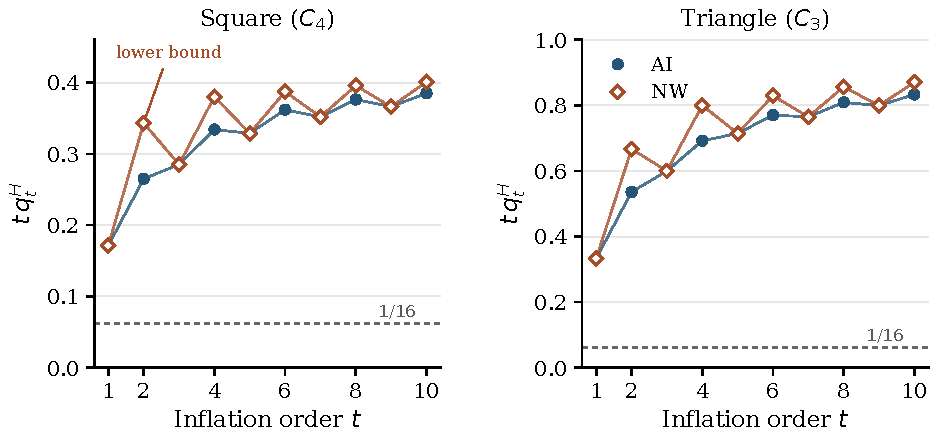
\includegraphics[width=\linewidth]{figures/thresholds.pdf}
\caption{Certified parity thresholds through order ten, rescaled by $t$. Markers show lower endpoints; two-sided brackets have width $4\cdot10^{-9}$ before rescaling. The square NW order-two point is a lower bound only. Dashed: the all-order guarantees $q=(16/15)^{2/t}-1$ and $q=(9/8)^{2/t}-1$ of Theorems~\ref{thm:squarelinear} and~\ref{thm:trianglelinear}. Panels use different vertical scales; connecting segments are visual aids only.}\label{fig:thresholds}
\end{figure}

